\section{Memory Banks}

  Now that we have established registers, we can use them to build arbitrary sets of memory. For example, by abstracting away the circuits and sticking a bunch of 1-bit registers together, we can get a sequence of them. The location of a register in this sequence is called the \textbf{memory address} of the register. 

  \begin{figure}[H]
    \centering 
    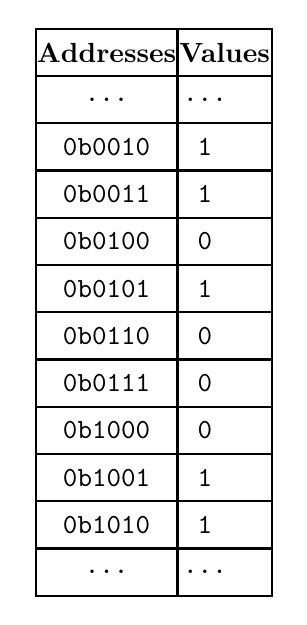
\begin{tikzpicture}
      % Draw the main table
      \draw[thick] (0,-1.2) rectangle (3,6.0);
      
      % Draw horizontal lines for rows
      \foreach \y in {-0.6,0,0.6,1.2,1.8,2.4,3.0,3.6,4.2,4.8,5.4} {
        \draw[thick] (0,\y) -- (3,\y);
      }
      
      % Draw vertical line to separate address and value columns
      \draw[thick] (1.8,-1.2) -- (1.8,6.0);
      
      % Headers
      \node at (0.9,5.7) {\textbf{Addresses}};
      \node at (2.4,5.7) {\textbf{Values}};
      
      % Top ellipsis row
      \node at (0.9,5.1) {\texttt{...}};
      \node at (2.15,5.1) {\texttt{...}};
      
      % Data rows
      \node at (0.9,4.5) {\texttt{0b0010}};
      \node at (0.9,3.9) {\texttt{0b0011}};
      \node at (0.9,3.3) {\texttt{0b0100}};
      \node at (0.9,2.7) {\texttt{0b0101}};
      \node at (0.9,2.1) {\texttt{0b0110}};
      \node at (0.9,1.5) {\texttt{0b0111}};
      \node at (0.9,0.9) {\texttt{0b1000}};
      \node at (0.9,0.3) {\texttt{0b1001}};
      \node at (0.9,-0.3) {\texttt{0b1010}};
      
      % Value column
      \node at (2.15,4.5) {\texttt{1}};
      \node at (2.15,3.9) {\texttt{1}};
      \node at (2.15,3.3) {\texttt{0}};
      \node at (2.15,2.7) {\texttt{1}};
      \node at (2.15,2.1) {\texttt{0}};
      \node at (2.15,1.5) {\texttt{0}};
      \node at (2.15,0.9) {\texttt{0}};
      \node at (2.15,0.3) {\texttt{1}};
      \node at (2.15,-0.3) {\texttt{1}};
      
      % Bottom ellipsis row
      \node at (0.9,-0.9) {\texttt{...}};
      \node at (2.15,-0.9) {\texttt{...}};
    \end{tikzpicture}
    \caption{You can visualize memory as a long array of boxes of bits, similar to PO boxes. Memory simply works as a bunch of bits in your computer with each bit having some memory address, which is also a bit. For example, the memory address \texttt{0b0010} (2) may have the bit value of \texttt{0b1} (1) stored in it. } 
  \end{figure}

  However, computers do not need this fine grained level of control on the memory, and they really work at the Byte level rather than the bit level. Therefore, we can visualize the memory as a long array of boxes indexed by \textit{Bytes}, with each value being a byte as well. In short, the memory is \textbf{byte-addressable}. In certain architectures, some systems are \textbf{word-addressable}, meaning that the memory is addressed by words, which are 4 bytes.\footnote{Note that in here the size of a word is 2 bytes rather than 4 as stated above. This is just how it is defined in some \texttt{x86} architectures.} 

  \begin{figure}[H]
    \centering 
    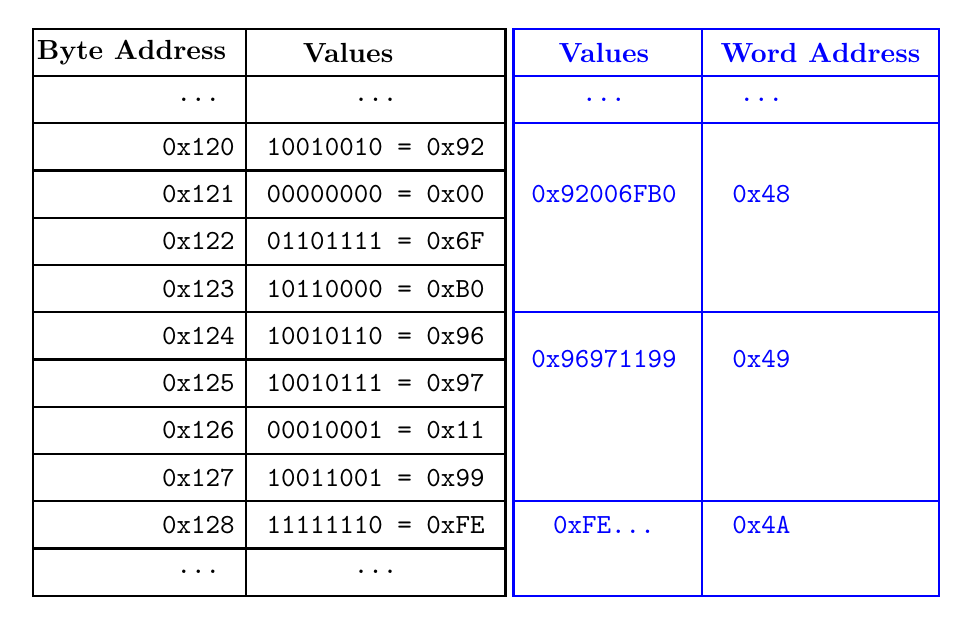
\begin{tikzpicture}
      % Draw the byte address table
      \draw[thick] (-1.5,-1.2) rectangle (4.5,6.0);
      
      % Draw horizontal lines for rows
      \foreach \y in {-0.6,0,0.6,1.2,1.8,2.4,3.0,3.6,4.2,4.8,5.4} {
        \draw[thick] (-1.5,\y) -- (4.5,\y);
      }
      
      % Draw vertical lines
      \draw[thick] (1.2,-1.2) -- (1.2,6.0);
      \draw[thick] (4.5,-1.2) -- (4.5,6.0);
      
      % Draw the word address table
      \draw[thick, blue] (4.6,-1.2) rectangle (10.0,6.0);
      
      % Draw horizontal lines for word table
      \foreach \y in {0,2.4,4.8,5.4} {
        \draw[thick, blue] (4.6,\y) -- (10.0,\y);
      }
      
      % Draw vertical line for word table
      \draw[thick, blue] (7,-1.2) -- (7,6.0);
      
      % Headers
      \node at (-0.25,5.7) {\textbf{Byte Address}};
      \node at (2.5,5.7) {\textbf{Values}};
      \node[blue] at (5.75,5.7) {\textbf{Values}};
      \node[blue] at (8.5,5.7) {\textbf{Word Address}};
      
      % Top ellipsis row
      \node at (0.6,5.1) {\texttt{...}};
      \node at (2.85,5.1) {\texttt{...}};
      \node[blue] at (5.75,5.1) {\texttt{...}};
      \node[blue] at (7.75,5.1) {\texttt{...}};
      
      % Byte addresses
      \node at (0.6,4.5) {\texttt{0x120}};
      \node at (0.6,3.9) {\texttt{0x121}};
      \node at (0.6,3.3) {\texttt{0x122}};
      \node at (0.6,2.7) {\texttt{0x123}};
      \node at (0.6,2.1) {\texttt{0x124}};
      \node at (0.6,1.5) {\texttt{0x125}};
      \node at (0.6,0.9) {\texttt{0x126}};
      \node at (0.6,0.3) {\texttt{0x127}};
      \node at (0.6,-0.3) {\texttt{0x128}};
      
      % Byte values
      \node at (2.85,4.5) {\texttt{10010010 = 0x92}};
      \node at (2.85,3.9) {\texttt{00000000 = 0x00}};
      \node at (2.85,3.3) {\texttt{01101111 = 0x6F}};
      \node at (2.85,2.7) {\texttt{10110000 = 0xB0}};
      \node at (2.85,2.1) {\texttt{10010110 = 0x96}};
      \node at (2.85,1.5) {\texttt{10010111 = 0x97}};
      \node at (2.85,0.9) {\texttt{00010001 = 0x11}};
      \node at (2.85,0.3) {\texttt{10011001 = 0x99}};
      \node at (2.85,-0.3) {\texttt{11111110 = 0xFE}};
      
      % Word values
      \node[blue] at (5.75,3.9) {\texttt{0x92006FB0}};
      \node[blue] at (5.75,1.8) {\texttt{0x96971199}};
      \node[blue] at (5.75,-0.3) {\texttt{0xFE...}};
      
      % Word addresses
      \node[blue] at (7.75,3.9) {\texttt{0x48}};
      \node[blue] at (7.75,1.8) {\texttt{0x49}};
      \node[blue] at (7.75,-0.3) {\texttt{0x4A}};
      
      % Bottom ellipsis row
      \node at (0.6,-0.9) {\texttt{...}};
      \node at (2.85,-0.9) {\texttt{...}};
    \end{tikzpicture}
    \caption{Visualization of memory as a long array of boxes of bytes. Every address is a byte and its corresponding value at that address is also a byte, though we represent it as a 2-digit hex. } 
    \label{fig:memory_visual_byte}
  \end{figure}

  \begin{definition}[Memory Bank]
    A \textbf{memory bank} with respect to an ISA is the smallest unit of addressable memory units. 
  \end{definition}

  It is intuitive to think that given some multi-byte object like an \texttt{int} (4 bytes), the beginning of the int would be the lowest address and the end of the int would be the highest address, like how consecutive integers are stored in an array. However, this is not always the case (almost always not the case since most computers are little-endian).  

  \begin{definition}[Endian Architecture]
    The \textbf{endianness} of an ISA refers to the byte order in which data is stored in memory. 
    \begin{enumerate} 
      \item A \textbf{big-endian architecture} (e.g. SPARC, z/Architecture) will store it so that the least significant byte has the highest address.
      \item A \textbf{little-endian architecture} (e.g. x86, x86-64, RISC-V) will store it so that the least significant byte has the lowest address. 
      \item A \textbf{bi-endian architecture} (e.g. ARM, PowerPC) can specify the endianness as big or little. 
    \end{enumerate}

    \begin{figure}[H]
      \centering 
      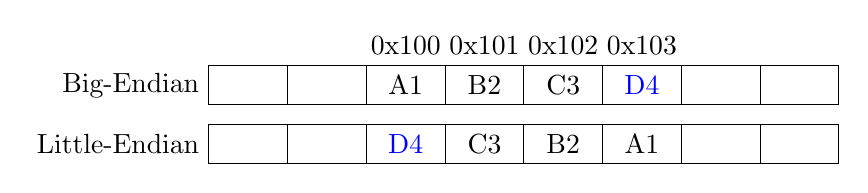
\begin{tikzpicture}[scale=0.5]
        \draw (-4, 0) rectangle (12, 1); 
        \draw (-4, 1.5) rectangle (12, 2.5); 
        \foreach \x in {-2, 0, 2, 4, 6, 8, 10} {
          \draw (\x, 0) -- (\x, 1);
          \draw (\x, 1.5) -- (\x, 2.5);
        }
        \node[left] at (-4, 0.5) {Little-Endian};
        \node[left] at (-4, 2) {Big-Endian};


        \node[blue] at (1, 0.5) {D4};
        \node at (3, 0.5) {C3};
        \node at (5, 0.5) {B2};
        \node at (7, 0.5) {A1};

        \node at (1, 2) {A1};
        \node at (3, 2) {B2};
        \node at (5, 2) {C3};
        \node[blue] at (7, 2) {D4};

        \node at (1, 3) {0x100};
        \node at (3, 3) {0x101};
        \node at (5, 3) {0x102};
        \node at (7, 3) {0x103};
      \end{tikzpicture}
      \caption{The big vs little endian architectures when storing 4-byte int data \texttt{0xA1B2C3D4} at address \texttt{0x100}.} 
      \label{fig:endianness}
    \end{figure}
  \end{definition}
  
  Note that endianness is not a property of memory, but a property of the ISA. 

  \begin{example}
    We can simply print out the hex values of primitive types to see how they are stored in memory, but it does not provide the level of details that we want on which bytes are stored where. At this point, we must use certain \textbf{debuggers} to directly look at the memory. For x86 architectures, we can use \texttt{gdb} and for ARM architectures, we can use \texttt{lldb}. At this point, we need to understand assembly to look through debuggers, so we will provide the example here. 
  \end{example}

  Let's clarify the differences between registers and memory banks. Memory is an overloaded term that is thrown as an umbrella term for any type of data storage, or as RAM. Memory is addressed by an unsigned integer while registers have names as we will see later (e.g. \texttt{\%rsi}). RAM is much bigger at several GB, while the total register space is much smaller at around a few KB at most. The memory is much slower than registers, which is usually on a sub-nanosecond timescale. The memory is dynamic and can grow as needed while the registers are static and cannot grow.

\subsection{Data Buses} 

  RAM gives us a large pool of memory to work with, albeit slow. 

\subsection{Fetching and Writing} 

  Getting memory addresses is not just multiplexers since its too slow. 


